\subsection{Wireless TCP}
Characteristics:
\begin{itemize}
    \item Problems:
    \begin{itemize}
        \item[$\rightarrow$] there are error losses $\rightarrow$ they are assumed
        as congestion $\Rightarrow$ Shrinked CWND $\Rightarrow$ drop data rate
        \item[$\rightarrow$] difficult to distinguish congestion from error losses
        \item[$\rightarrow$] there are burst losses $\Rightarrow$ multiple CWND
        shrinking $\Rightarrow$ drop data rate
        \item[$\rightarrow$] there is latency $\rightarrow$ it can be:
        \begin{itemize}
            \item variable
            \item hard to estimate $\rightarrow$ $\frac{\text{RTT}}{\text{RTO}}$
            \item high $\rightarrow$ protocol no more fair
        \end{itemize}
        \item[$\rightarrow$] there can be disconnections/handoff/fading $\rightarrow$
        for weaker signal
        \item[$\rightarrow$] bandwidth can be variable $\Rightarrow$ wastage and loss bursts
    \end{itemize}
    \item Multi-Hop Wireless Paths:
    \begin{itemize}
        \item[$\rightarrow$] there is an exponential decrease of throughput/ increased delay\\
        $\rightarrow$ from 1 to 3 hops
        \item[$\rightarrow$] packets/transmissions are in competition\\
        $\rightarrow$ contention also between datas and ACKs $\rightarrow$ if channel is
        not free\\$\Rightarrow$ waiting
        \item[$\rightarrow$] lareger number of hops $\Rightarrow$ throughput stabilizes
        $\rightarrow$ effective pipelining 
    \end{itemize}
    \item Throughput decrease:
    \begin{itemize}
        \item[$\rightarrow$] generally true when increasing speed
        \item[$\rightarrow$] why $\rightarrow$ because of link breakage and repair latency:
        \begin{enumerate}
            \item sender doesn't know that the link is broken\\
            $\Rightarrow$ it may continue transmitting (packet loss)
            \item sender doesn't know when it is all available again\\
            $\rightarrow$ it will retransmit when timeout occurs
        \end{enumerate}
        \item[$\rightarrow$] how to improve it:
        \begin{itemize}
            \item network feedback $\rightarrow$ if AWND of receiver has size 0,
            network can notify sender $\Rightarrow$ sender stops immediately
            \item TCP failure $\rightarrow$ sender is notified with a message about it
            \item TCP callback $\rightarrow$ let sender knows when link is broken/repaired
            \item dynamic TCP timeout $\rightarrow$ alleviate TCP timeouts/backoffs
        \end{itemize}
    \end{itemize}
\end{itemize}
\newpage
\subsubsection{Wireless TCP Protocols}
There are different types of protocols for transport layers in wireless TCP:
\begin{itemize}
    \item Connection split:
    \begin{itemize}
        \item[$\rightarrow$] local retransmission
        \item[$\rightarrow$] quick action on wireless link
        \item[$\rightarrow$] TCP specific for wireless link
        \item[$\rightarrow$] Examples:\\[0.15cm]
        \begin{minipage}{0.3 \textwidth}
            \begin{itemize}
                \item I-TCP
                \item PROXY
            \end{itemize}
        \end{minipage}
        \begin{minipage}{0.3 \textwidth}
            \begin{itemize}
                \item M-TCP
                \item SNOOP
            \end{itemize}
        \end{minipage}
    \end{itemize}
    \item Pure End-to-End:
    \begin{itemize}
        \item[$\rightarrow$] new protocol $\rightarrow$ better than old version, retrocompatibility \dots
        \item[$\rightarrow$] sender is aware of wireless link
        \item[$\rightarrow$] Examples:\\[0.15cm]
        \begin{minipage}{0.3 \textwidth}
            \begin{itemize}
                \item Delayed Dupacks
                \item Freeze-TCP
                \item WTCP
                \item TCP Hybla
                \item TCP High Speed
                \item TCP Fast
            \end{itemize}
        \end{minipage}
        \begin{minipage}{0.3 \textwidth}
            \begin{itemize}
                \item TCP-Aware
                \item TCP Probing
                \item TCP Westwood
                \item TCP CUBIC
                \item TCP Compound
                \item \dots
            \end{itemize}
        \end{minipage}
    \end{itemize}
\end{itemize}
Here there are a description of some of them.

\paragraph{SNOOP Protocol} \mbox{}\\[0.2cm]
Characteristics:
\begin{itemize}
    \item it is designed to address high BER
    \item Base Station implements a Snoop Agent
    \begin{itemize}
        \item[$\rightarrow$] it monitors all packets of sender and receiver (also ACKs)
        \item[$\rightarrow$] it caches packets not acked yet into base station
        \item[$\rightarrow$] it intercepts dupacks:
        \begin{itemize}
            \item $\frac{1}{2}$ $\rightarrow$ immediate retranssmission (sender not notified)
            \item 3 $\rightarrow$ let sender knows about it (CWND shrinkage)
        \end{itemize}
    \end{itemize}
    \item Path: sender $\Leftrightarrow$ snoop agent $\Leftrightarrow$ receiver
    \item it needs low latency between sender and snoop agent\\$\Rightarrow$
    otherwise traditional TCP is better
    \item Pro:
    \begin{itemize}
        \item[$\tikzcmark$] End-to-End preservation $\rightarrow$ no ACK created by snoop agent
        \item[$\tikzcmark$] local retransmission
        \item[$\tikzcmark$] high BER address 
    \end{itemize}
    \item Cons:
    \begin{itemize}
        \item[$\tikzxmark$] requirement of little latency on the wireless link
        \item[$\tikzxmark$] same performances on long disconnections
        \item[$\tikzxmark$] immediately after a handoff $\Rightarrow$ Slow Start $\rightarrow$
        no packets in new cache
    \end{itemize}
\end{itemize}

\paragraph{Satellites}\mbox{}\\[0.2cm]
There are:
\begin{itemize}
    \item GEO $\rightarrow$ have backbone configuration $\rightarrow$ so there is\\
    $\Rightarrow$ bridge between terrestrial antenna
    \item LEO $\rightarrow$ have direct to home configuration $\rightarrow$ so it works as\\
    $\Rightarrow$ (terrestrial antenna $\rightarrow$ satellite $\rightarrow$ home)
\end{itemize}
All of them have:
\begin{itemize}
    \item high RTT $\rightarrow$ it can be $\approx$ 600ms for GEO
    \item important PER\footPER $\rightarrow$ due to radio channels $\rightarrow$
    interferences, wheather \dots
\end{itemize}

\paragraph{Slow Start and Congestion Avoidance Models}\mbox{}\\[0.2cm]
Characteristics:
\begin{itemize}
    \item also referred as Van Jacobson algorithm
    \item In Slow Start phase:
    \begin{itemize}
        \item[$\rightarrow$] CWND $=$ CWND $+$ 1 for every new ACK received
        \item[$\rightarrow$] CWND $=$ 2 $\cdot$ CWND for every RTT
    \end{itemize} 
    \item In Congestion Avoidance phase:
    \begin{itemize}
        \item[$\rightarrow$] CWND $=$ CWND $+$ $\frac{\text{1}}{\text{CWND}}$ for every new
        ACK received
        \item[$\rightarrow$] CWND $=$ 2 $\cdot$ CWND for every RTT
    \end{itemize}
    \item RTT changes dynamically
    \begin{figure}[!h] 
        \centering 
        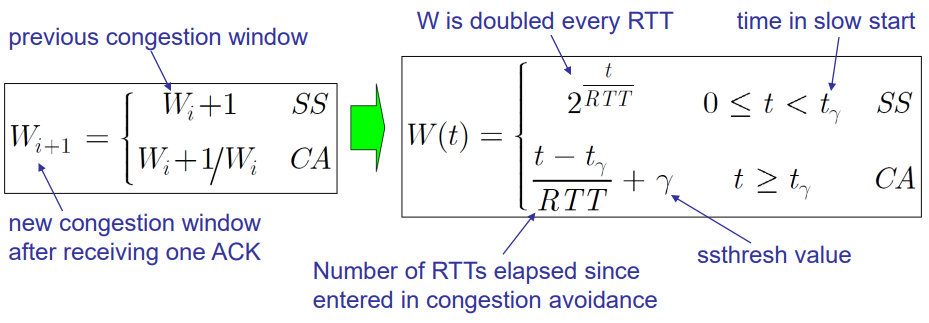
\includegraphics[scale = 0.37]{images/ss-ca-formulas.png} 
        \caption{Slow Start \& Congestion Avoidance Models}
        \label{ss-ca-formulas}
    \end{figure}
\end{itemize}

\paragraph{RTT Unfairness}\mbox{}\\[0.2cm]
It is one of the problems that protocols have to solve:
\begin{itemize}
    \item B(t) $=$ $\frac{\text{W(t)}}{RTT}$ $\Rightarrow$ where B(t) $=$ bandwidth and 
    W(t) $=$ window growth rate
    \item longer RTT $\Rightarrow$ slower phase growth rate
    \item smaller RTT $\Rightarrow$ bigger bandwidth
\end{itemize}

\paragraph{TCP Hybla}\mbox{}\\[0.2cm]
Characteristics:
\begin{itemize}
    \item it equalizes transmission rate against RTT $\Rightarrow$ fair RTT
    \item a longer RTT $\Rightarrow$ compensate by sending twice on every ACK
    ($\neq$ every RTT)
    \item there is the introduction of parameter $\rho$ $=$
    $\frac{\text{RTT}}{\text{RTT}_\text{0}}$ where:
    \begin{itemize}
        \item[$\rightarrow$] RTT is actual Round Trip Time
        \item[$\rightarrow$] $\text{RTT}_\text{0}$ is reference Round Trip Time (for example
        $\text{RTT}_\text{0}$ $=$ 25ms)
    \end{itemize}
    \begin{figure}[!h] 
        \centering 
        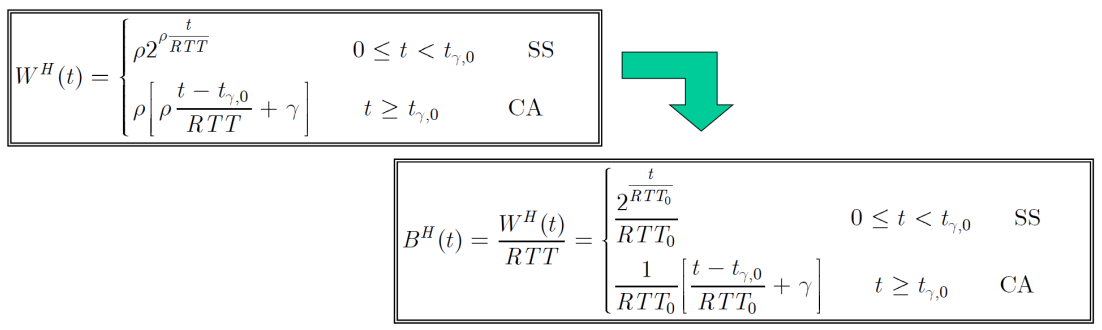
\includegraphics[scale = 0.3]{images/ss-ca-hybla.png} 
        \caption{Slow Start \& Congestion Avoidance for TCP Hybla}
        \label{ss-ca-hybla}
    \end{figure}
    \item Pros:
    \begin{itemize}
        \item[$\rightarrow$] End-to-End solution
        \item[$\rightarrow$] it changes only on sender side $\Rightarrow$ easily deployable\\
        $\rightarrow$ no damage for the entire system 
        \item[$\rightarrow$] it has RTT fairness
    \end{itemize}
    \item Cons:
    \begin{itemize}
        \item[$\rightarrow$] it is so aggressive $\Rightarrow$ it can lead to multiple losses
        \item[$\rightarrow$] measured RTT is sensitive to buffer size $\rightarrow$ limited and not sustainable anymore at a certain point
        \item[$\rightarrow$] no handling on BER/disconnections (as most of TCPs)
        \item[$\rightarrow$] doubts about friendliness and fairness
    \end{itemize}
\end{itemize}
What is friendliness:
\begin{itemize}
    \item how different flows of TCPs cooperate
    \begin{itemize}
        \item[$\rightarrow$] total amount of bandwidth increased
        \item[$\rightarrow$] average amount of bandwidth
    \end{itemize}
    \item new version shouldn't steal bandwidth of older versions\\$\rightarrow$ it can
    take all new available bandwidth
\end{itemize}

\paragraph{TCP Westwood \& TCP Westwood Plus}\mbox{}\\[0.2cm]
Characteristics:
\begin{itemize}
    \item it is pure End-to-End
    \item flow control is based on estimation of eligible bandwidth (BWE)
    \begin{itemize}
        \item[$\rightarrow$] monitoring of acks' arrival rate at sender side
        \item[$\rightarrow$] use of BWE to set CWND and SSThresh after a loss
        \begin{itemize}
            \item 3 Dupacks:
            \begin{itemize}
                \item SSThresh $=$ BWE $\cdot$ $\text{RTT}_{\text{min}}$
                ($\neq$ TCP New Reno $\rightarrow$ SSThresh $=$ $\frac{\text{CWND}}{\text{2}}$)
                \item if CWND > SSThresh $\Rightarrow$ CWND $=$ SSThresh
            \end{itemize}
            \item Timeout expiration:
            \begin{itemize}
                \item SSThresh $=$ BWE $\cdot$ $\text{RTT}_{\text{min}}$
                ($\neq$ TCP New Reno $\rightarrow$ SSThresh $=$ $\frac{\text{CWND}}{\text{2}}$)
                \item CWND $=$ 1
            \end{itemize}
        \end{itemize}
        \item[$\rightarrow$] sending more than what you receive won't affect BWE
    \end{itemize}
    \begin{figure}[!h] 
        \centering 
        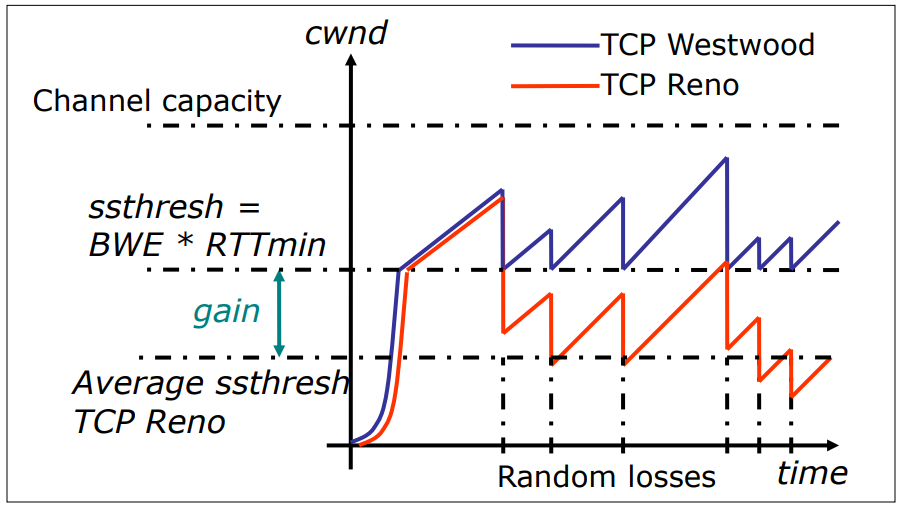
\includegraphics[scale = 0.37]{images/westwood-vs-reno.png} 
        \caption{TCP Westwood vs TCP Reno}
        \label{westwood-vs-reno}
    \end{figure}
    \newpage
    \item Rate Estimation:
    \begin{itemize}
        \item[$\rightarrow$] useful to enhance congestion control
        \item[$\rightarrow$] computed by sampling/exponential filtering at sender
        \item[$\rightarrow$] based on ACKs arrival times and amount of bandwidth delivered\\
        $\Rightarrow$ data ACKed are aggregated in interval T $=$ RTT
        \item[$\rightarrow$] used by sender to set CWND and SSThresh
    \end{itemize}
    \item Pros:
    \begin{itemize}
        \item BWE allows to reach higher throughput
        \item it changes only on sender side
    \end{itemize}
    \item Cons:
    \begin{itemize}
        \item wrong BWE over asymmetric links
        \item No handling of high BER/disconnections
        \item doubts about friendliness and fairness
    \end{itemize}
\end{itemize}

\paragraph{TCP Adaptive Selection}\mbox{}\\[0.2cm]
Characteristics:
\begin{itemize}
    \item possibility to have different TCP variants concurrently
    $\rightarrow$ matching different characteristics of connections
    \item it can be applied in different ways depending on:
    \begin{itemize}
        \item[$\rightarrow$] agent that performs TCP selection
        \item[$\rightarrow$] use of cross-layer approach $\Rightarrow$ not linked by the standard
        \item[$\rightarrow$] changing TCP version on on-going connection $\Rightarrow$ dynamic selection
    \end{itemize}
    \item there are different modules that can be replaced in TCP-module-container\\
    $\rightarrow$ criteria:
    \begin{itemize}
        \item[$\rightarrow$] TCP parameters $\rightarrow$ RTT, BWE \dots
        \item[$\rightarrow$] cross-layer informations
        \item[$\rightarrow$] reliable channel estimation
    \end{itemize}
\end{itemize}

\paragraph{TCP Cubic}\mbox{}\\[0.2cm]
Characteristics:
\begin{itemize}
    \item it is used by default in linux kernels
    \item optimized congestion control algorithm for high speed networks with high latency
    \item window $\rightarrow$ cubic function of time since last congestion event
    \item Algorithm:
    \begin{enumerate}
        \item inflection point set CWND prior last congestion event
        \item quickly initial growth
        \item slow down + stay stable around CWND value when congestion happens
        \item no loss happens $\rightarrow$ quickly growth again
    \end{enumerate}
    \item Differences with standard TCPs
    \begin{itemize}
        \item[$\rightarrow$] TCP Cubic doesn't rely on receipt of ACKs to increase CWND
        \item[$\rightarrow$] TCP Cubic's CWND depends only on the last congestion event\\
        $\Rightarrow$ less RTT-unfairness $\rightarrow$ window growth independent from RTT
    \end{itemize}
\end{itemize}
\begin{figure}[!h] 
    \centering 
    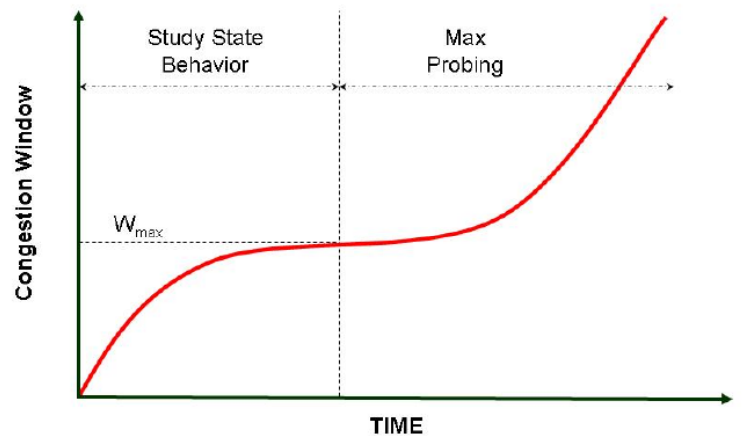
\includegraphics[scale = 0.4]{images/cwnd-growth-tcp-cubic.png} 
    \caption{TCP Cubic: CWND growth}
    \label{cwnd-growth-tcp-cubic}
\end{figure}